\documentclass[spanish,12pt,letterpapper]{article}
\usepackage{babel}
\usepackage[utf8]{inputenc}
\usepackage{graphicx}
\usepackage{mathtools}
\begin{document}
	\begin{titlepage}
		\begin{center}
			
\includegraphics[width=0.6\textwidth]{../logoUnADM}~\\[1cm] 
			\textsc{Universidad Abierta y a Distancia de México}\\[0.8cm]
			\textsc{Desarrollo de Software}\\[1.8cm]
			
			\textbf{ \Large Actividad 1. Problemas de álgebra y cálculo  }\\[3cm]
			
			Diego Antonio Plascencia Lara\\ ES1421004131 \\[0.4cm]
			Facilitador(a): CESAR ALEXIE CHAN PUC  \\
			Materia: Diseño de Bases de Datos\\
			Grupo: DS-DDBD-1601-B1-003 \\
			Unidad: III \\
			
			\vfill México D.F\\{\today}
			
		\end{center}
	\end{titlepage}
	
	\section{Planteamiento del Problema}	
	''Se desea diseñar una base de datos para almacenar y gestionar la información empleada por una empresa dedicada a la venta de automóviles, teniendo en cuenta los siguientes aspectos:\\
	
	La empresa dispone de una serie de coches para su venta. Se necesita conocer el número de serie, marca y modelo, el color y el precio de venta de cada coche, incluye también las placas. Los datos que interesa conocer de cada cliente son el número de IFE, nombre, dirección, ciudad y número de teléfono: además, los clientes se diferencian por un código interno de la empresa que se incrementa automáticamente cuando un cliente se da de alta en ella. Un cliente puede comprar tantos coches como desee a la empresa. Un coche determinado solo puede ser comprado por un único cliente.El concesionario también se encarga de llevar a cabo las revisiones que se realizan a cada coche. Cada revisión tiene asociado un código que se incrementa automáticamente por cada revisión que se haga. De cada revisión se desea saber si se ha hecho cambio de filtro, si se ha hecho cambio de aceite, si se ha hecho cambio de frenos u otros. Los coches pueden pasar varias revisiones en el concesionario.``\\
	
	\subparagraph{Puntos a tratar}
	\begin{itemize}
	\item Instala en tu pc el SGBD que investigaste en la unidad 1.
	\item Elaborar el modelo entidad-relación del caso.
	\item Identifica las entidades, atributos y sus características.
	\item Crea la base de datos en el SGBD con el nombre AUTO\_INICIALES\_UNI3EJE1.
	\end{itemize}
	
	\section{Análisis de las Operaciones relacionales.}
	\subsection{Instalación DBMS}
	\begin{center}
	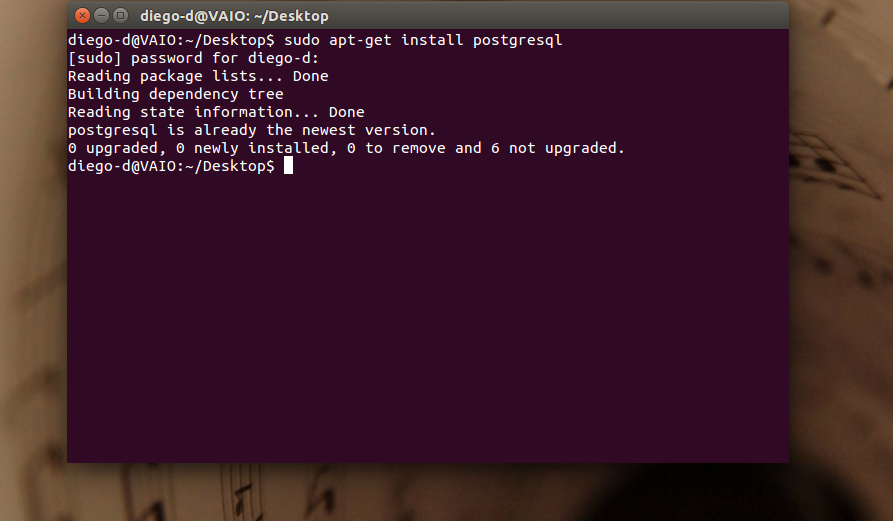
\includegraphics[width=0.7\textwidth]{./images/a}~\\[1cm]
	\end{center}
	
	La captura es de la terminal ejecutando el comando para instalar por administrador de paquetes postgresql, pero indica que ya lo tengo y que no necesita actualizarse, por que lo hice en el ejercicio anterior.
    	
	\subsection{Modelo entidad-relación}
	\begin{center}
	\includegraphics[width=0.8\textwidth]{./images/b}~\\[1cm]
	\end{center}
	
	Es el modelo entidad-relación retomado del primer ejercicio de la unidad 2, con sus atributos y relaciones, así como los identificadores que son las llaves primarias de las entidades señaladas con gris.
	
	\subsection{Entidades y atributos}
	\begin{center}
	\begin{tabular}{| p{4cm} | p{4cm} |}
	\hline
	
	\textbf{Entidad} & \textbf{Atributos}\\
	\hline
	Car & serial\_no (pk): varchar(64)*\linebreak brand: varchar(24)* \linebreak model: varchar(32)* \linebreak color: varchar(16)* \linebreak price: numeric(11,2)* \linebreak plates: varchar(8) \linebreak customer\_id (fk): bigint\\
	\hline
	Custumer & id (pk): bigserial \linebreak ife: bigint  \linebreak name: varchar(64) \linebreak address: text \linebreak city: varchar(32) \linebreak tel: bigint \\
	\hline
	Inspection & id (pk): bigserial \linebreak filter\_chg: boolean \linebreak oil\_chg: boolean  \linebreak brakes\_chg: boolean \linebreak other\_chg: boolean \linebreak car\_serial\_no (fk): varchar(64)* \\
	
	\hline	
	\end{tabular}
	\end{center}
	
	En esta tabla se muestran las entidades mencionadas en la actividad, con sus respectivos atributos, de igual forma se muestra el tipo de dato de cada atributo, si son llaves primarias o foráneas y si son o no requeridos.
	
	\subsection{Creación de la Base de Datos}
	\begin{center}
	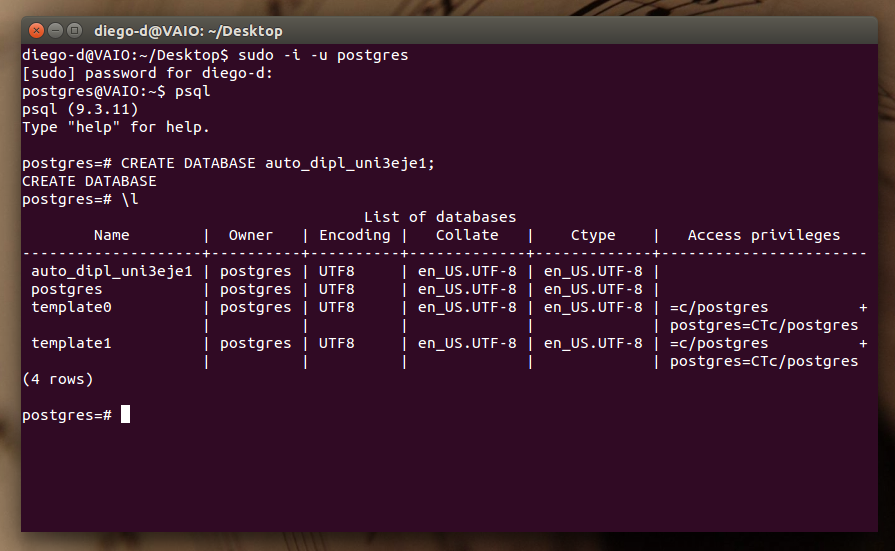
\includegraphics[width=0.8\textwidth]{./images/d}~\\[1cm]
	\end{center}
	Aquí se muestra la sentencia de SQL que interpreta postgreSQL para crear la base de datos, y un comando para listar todas las bases de datos en el DBMS;
	
	\subsection{Creación de Tablas}
	\begin{center}
	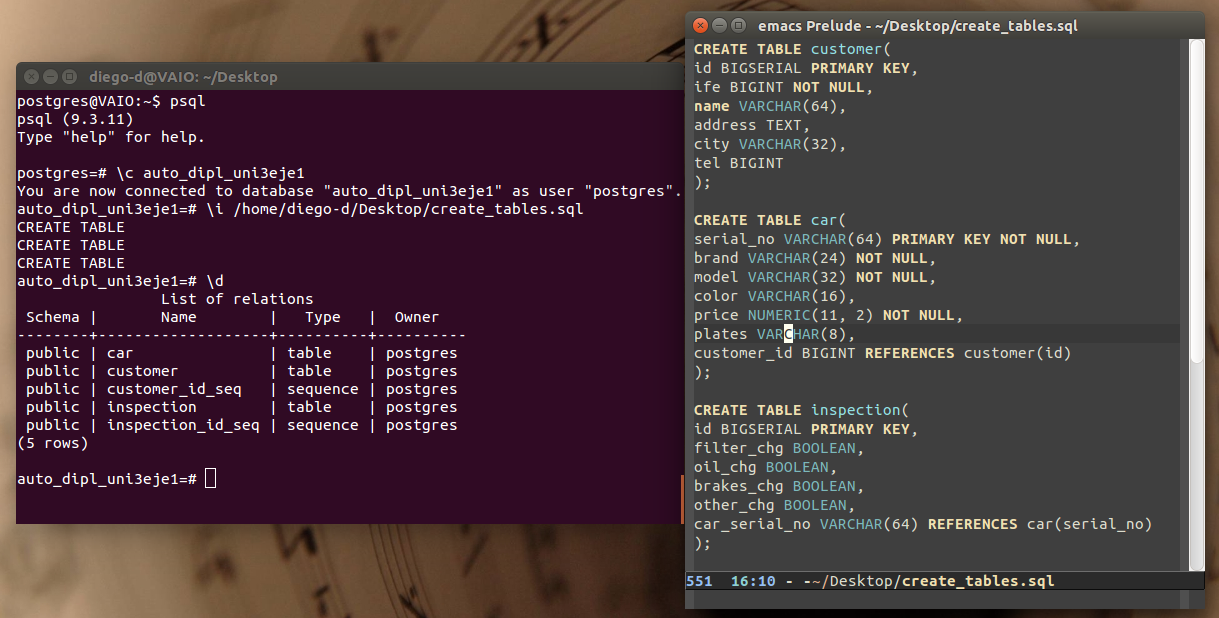
\includegraphics[width=0.8\textwidth]{./images/e}~\\[1cm]
	\end{center}
	Se implementa el modelo creando las tablas, del lado derecho se encuentra el script SQL para la creación de las tablas y del lado izquierdo se muestra el comando para ejecutarlo y para listas todas las tablas en nuestra DB;
	
	\subsection{Entrada de registros}
	\begin{center}
	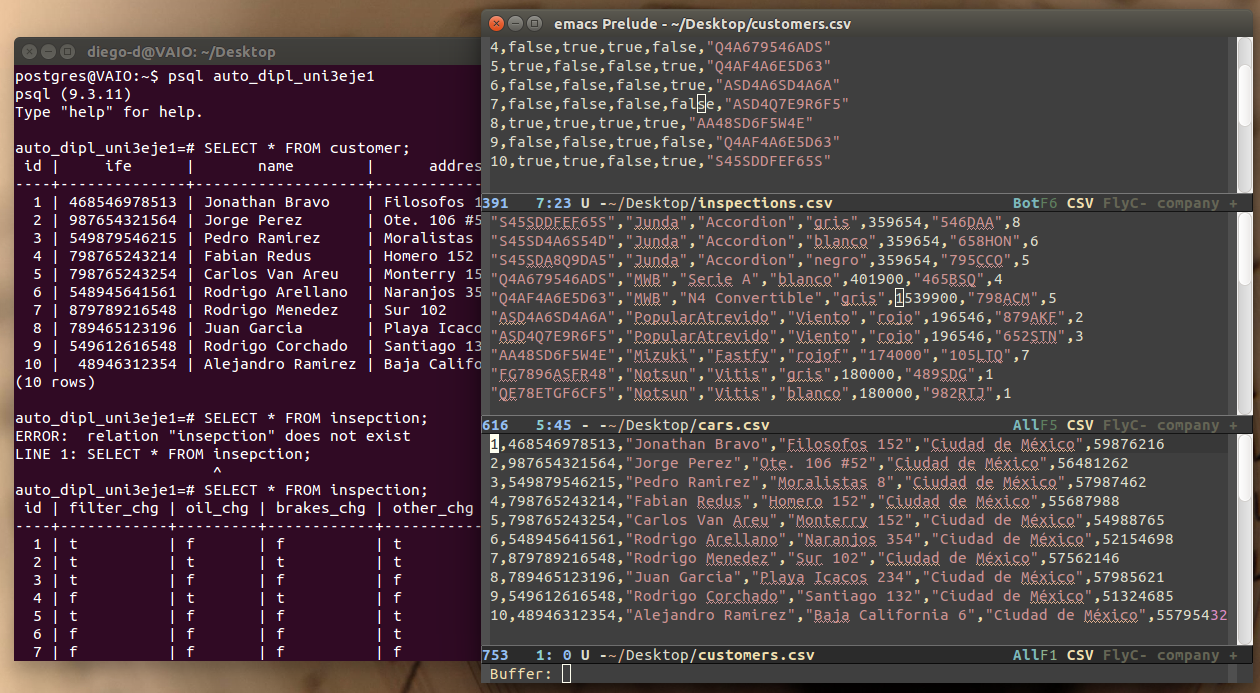
\includegraphics[width=0.8\textwidth]{./images/f}~\\[1cm]
	\end{center}
	En esta captura del lado derecho se encuentran los CSV completos con todos los datos a ingresar en la DB, del lado izquierdo se muestra la sentencia SQL para introducirlos y para mostrar la información de las tablas parcialmente.
	
	\section{Diseño Algebraico y Consultas.}
	
	\subsection{Unión clientes-autos}
	\begin{center}
	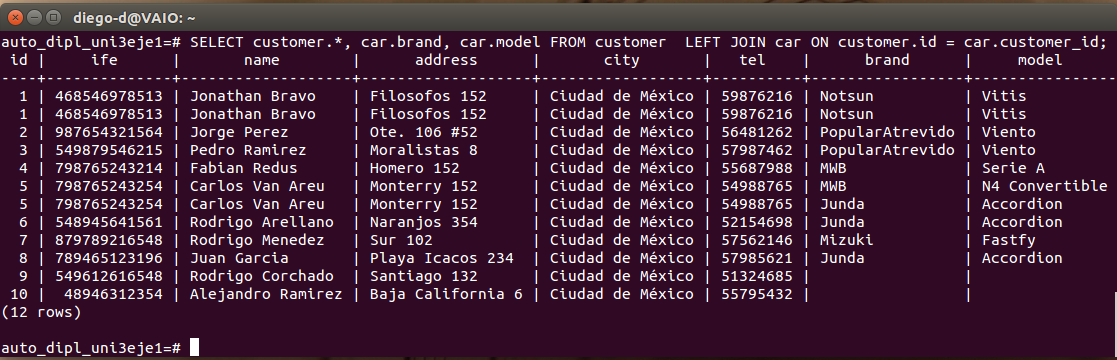
\includegraphics[width=0.8\textwidth]{./images/g}~\\[1cm]
	\end{center}
	Aquí se muestra la información de los clientes así como los autos que poseen (marca y modelo). Se hizo un left join, puesto que se pide la información de los clientes, pero puede que estos no tengan autos.\\
	
	Notacion algebraica: Car * Customer
	
	\subsection{Unión clientes-revisión}
	\begin{center}
	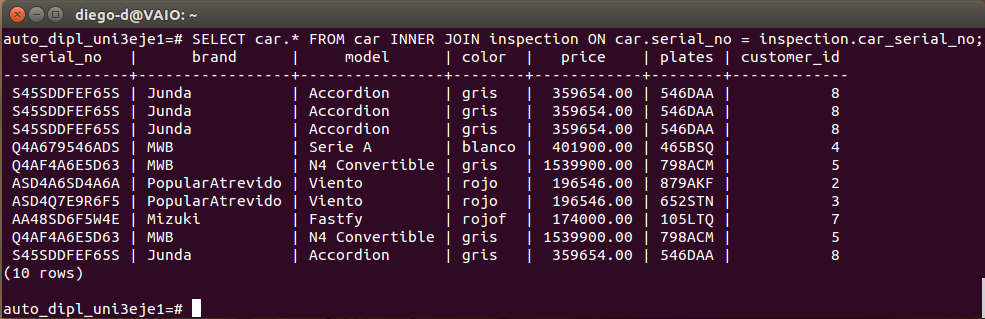
\includegraphics[width=0.8\textwidth]{./images/h}~\\[1cm]
	\end{center}
	Se muestra la información de los autos que han ingresado al taller. Se realizo un inner join, puesto que solo se necesita la información de los carros, pero este (su numero de serie) debe encontrarse en ambas tablas y solo se mostraran los que si.\\
	
	Notación algebraica: Car \(\cap\) Inspection
	
	\subsection{Selección clientes}
	\begin{center}
	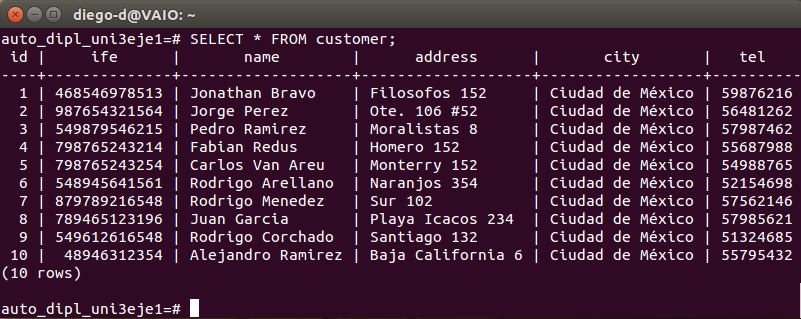
\includegraphics[width=0.8\textwidth]{./images/i}~\\[1cm]
	\end{center}
	Se observa la información de los clientes, esta información incluye sus IFEs. Se utilizo un simple query de selección, puesto que no especifica alguna condición.\\
	
	Notación algebraica:  \(\sigma\)Customer
	
	\section{Conclusiones}
	En mi opinión, el tema de álgebra y calculo en las BD es mas importante teóricamente y útil para el área de investigación y ciencia de datos, puesto que la extracción de datos denotada en álgebra es poco útil a la hora de la practica, ya que en mi caso no lo he llegado a usar.
	
	
	\pagebreak
	\begin{thebibliography}{9}	
	
	\bibitem{psqldocs} The PostgreSQL Development Team. 
		\emph{PostgreSQL 7.0 Docs}. PostgreSQL, [Disponible en: http://www.postgresql.org/docs/7.0/static/postgres.htm].
	
		\bibitem{rrhopkins} Robert J. Robbins. 
		\emph{Database Fundamentals}. Johns Hopkins University, [Disponible en: http://www.esp.org/db-fund.pdf].
		
		\bibitem{elmasriynavathe} Ramez Elmasri and Shamkant Navathe. 
		\emph{Fundamentals of Database Systems}. Pearson Education, [Disponible en: http://tinman.cs.gsu.edu/~raj/4710/f11/Ch01.pdf].

	\end{thebibliography}

\end{document}
